\hypertarget{jill-goodacre}{%
\section{Jill Goodacre}\label{jill-goodacre}}

\begin{figure}[!ht]
  \begin{adjustwidth}{-\oddsidemargin-1in}{-\rightmargin}
    \centering
    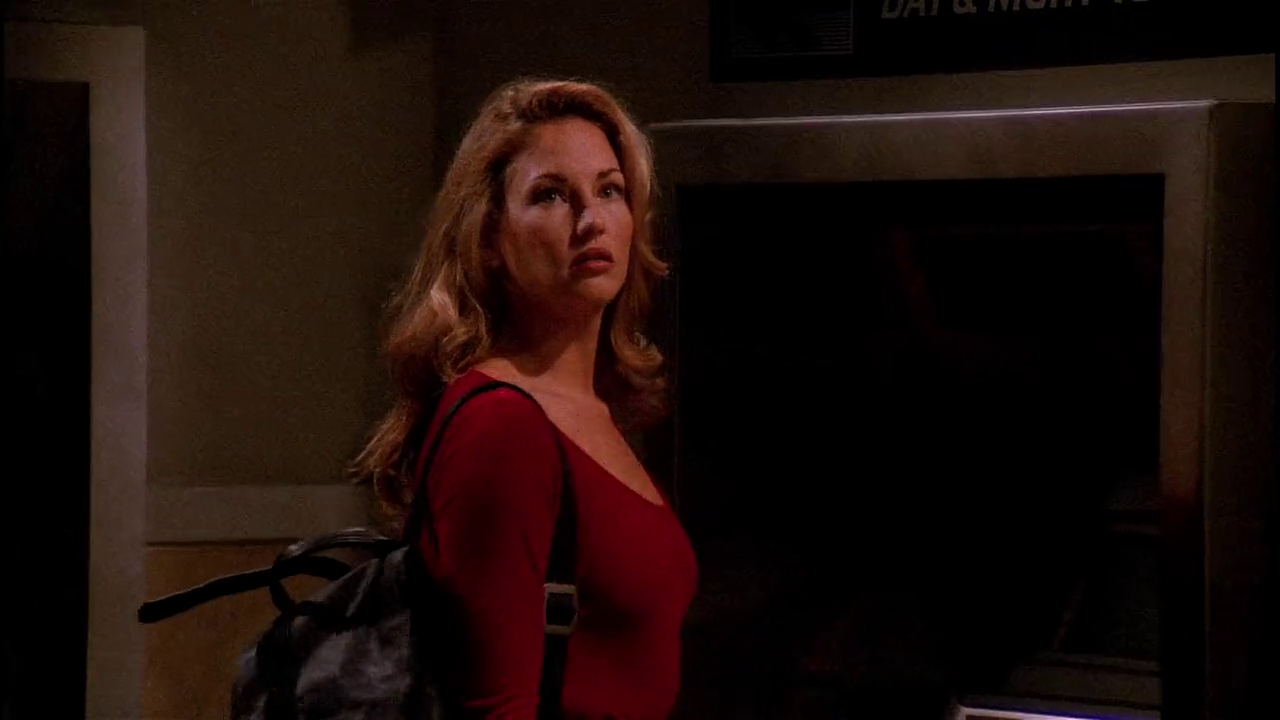
\includegraphics[trim={0 11cm 0 2cm,}, clip, width=\paperwidth]{./S01/img/7/jill-goodacre.png}
    % \caption{Jill Goodacre\label{fig:jill-goodacre}}
  \end{adjustwidth}
\end{figure}

\begin{tcolorbox}[enhanced,center upper,
    drop fuzzy shadow southeast, boxrule=0.3pt,
    lower separated=false, breakable,
    colframe=black!30!dialogoBorder,colback=white]
\begin{minipage}[c]{0.16\linewidth}
  \raisebox{\dimexpr-\height+\ht\strutbox\relax}{
    \centering 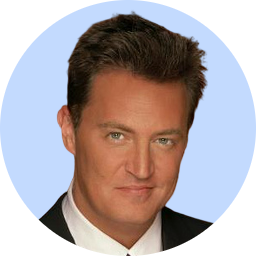
\includegraphics[width=1.4cm]{./assets/img/chandler.png}
  }
   & \centering \scriptsize{Chandler}
\end{minipage}
\hfill
\begin{minipage}[c]{0.8\linewidth}
  \textbf{- I am trapped in an ATM vestibule with Jill Goodacre.}\\
  - Estou preso num caixa 24 horas com Jill Goodacre.
\end{minipage}
\end{tcolorbox}

Ao ficar preso no banco devido ao blecaute, Chandler se vê acompanhado
da modelo e atriz \emph{Jill Goodacre} (1964), que foi uma das modelos
principais da \emph{Victoria's Secret} nos anos 80 e começo dos
90.\footnote{\sloppy Jill Goodacre - IMDB. \url{https://www.imdb.com/name/nm0004969/}}

\hypertarget{top-of-the-world}{%
\section{Top of the World}\label{top-of-the-world}}

\begin{figure}[!ht]
  \begin{adjustwidth}{-\oddsidemargin-1in}{-\rightmargin}
    \centering
    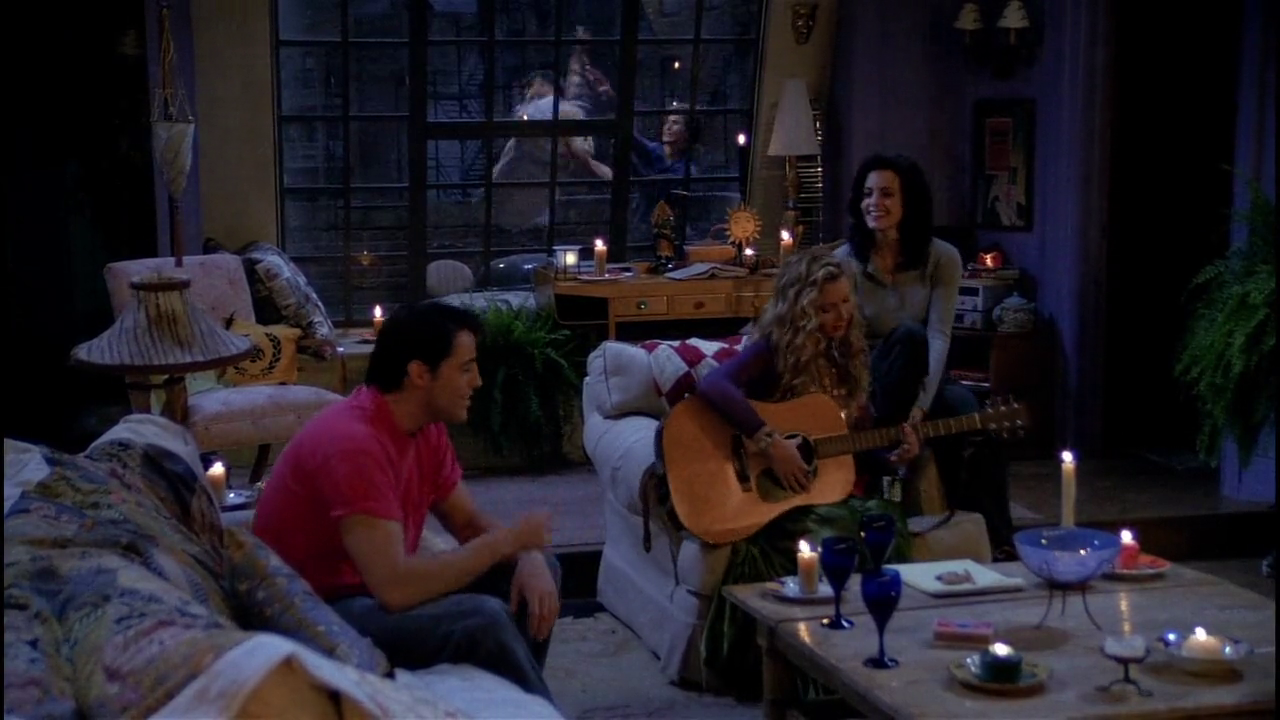
\includegraphics[trim={0 7cm 0 2cm,}, clip, width=\paperwidth]{./S01/img/7/top-of-the-world.png}
    % \caption{Top of the World\label{fig:top-of-the-world}}
  \end{adjustwidth}
\end{figure}

Enquanto Ross tenta se declarar para Rachel e é atacado pelo gato do
Paolo, os amigos Monica, Joey e Phoebe cantam a música \emph{Top of the
World} (1972) do \emph{The Carpenters}. Segue o trecho cantado pelos
três: \footnote{\sloppy Top of the World - YouTube. \url{https://www.youtube.com/watch?v=vupwAFMXLkA}}

\bigskip
\begin{tcolorbox}[enhanced,
    drop fuzzy shadow southeast, boxrule=0.3pt,
    lower separated=false, sidebyside, sidebyside align=top,
    halign=flush right, halign lower=left, breakable,
    colframe=black!30!dialogoBorder,colback=musicaBg]
\includegraphics[width=0.4cm]{./assets/img/icon-music.png}\\
I’m on the top of the world looking\\Down on creation and the only explanation I can find\\Is the love that I’ve found, ever since you’ve been around\\Your love’s put me at the top of the world\\
\tcblower
\includegraphics[width=0.4cm]{./assets/img/icon-language.png}\\
Eu estou no topo do mundo vendo\\Toda a criação lá embaixo e a única explicação que eu acho\\É que o amor que eu encontrei desde que você chegou\\Seu amor me colocou no topo do mundo\\
\end{tcolorbox}

Essa deve ser a única música que a Phoebe canta que não seja autoral ou
que não seja uma versão, por assim dizer.\footnote{\sloppy Top of the World - Letra. \url{https://www.letras.mus.br/carpenters/7023/traducao.html}}

\hypertarget{monopoly}{%
\section{Monopoly}\label{monopoly}}

\begin{figure}[!ht]
  \begin{adjustwidth}{-\oddsidemargin-1in}{-\rightmargin}
    \centering
    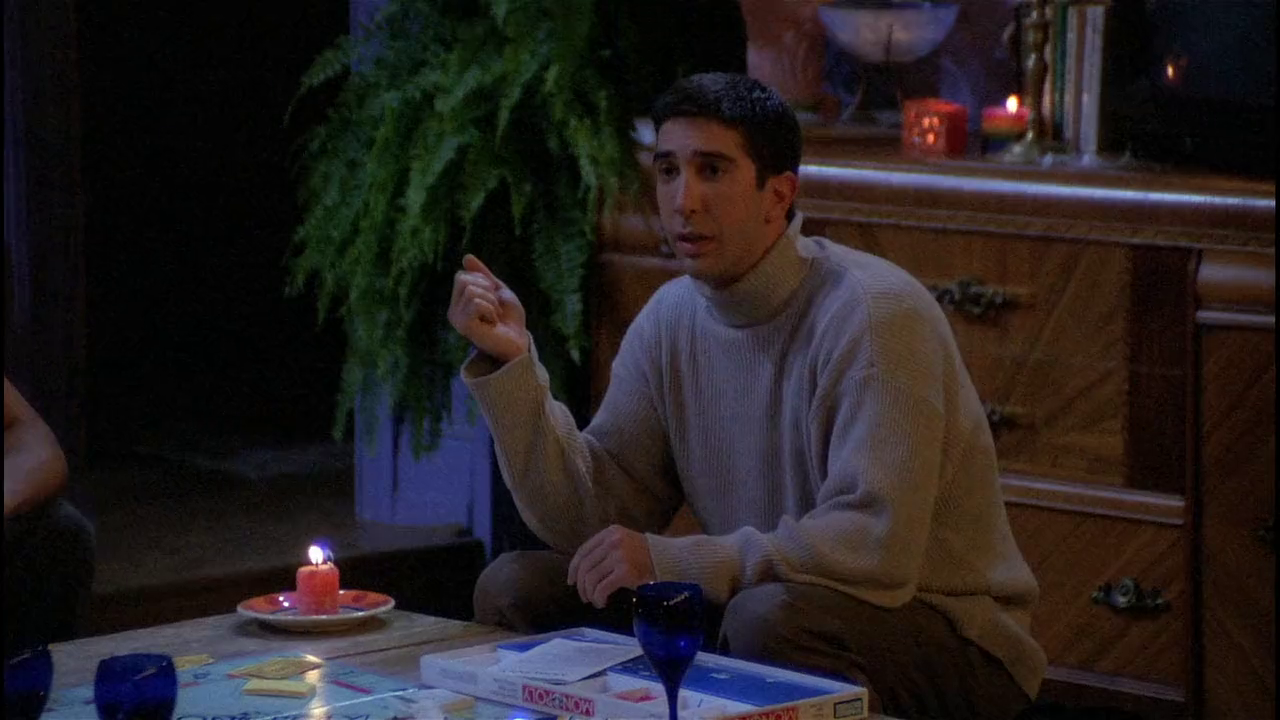
\includegraphics[trim={0 0cm 0 4cm,}, clip, width=\paperwidth]{./S01/img/7/monopoly.png}
    % \caption{Monopoly\label{fig:monopoly}}
  \end{adjustwidth}
\end{figure}

Enquanto esperam o blecaute passar, os amigos jogam \emph{Monopoly}
(1935), jogo de tabuleiro onde os jogadores devem se mover por meio do
lançamento de 2 dados de 6 faces, comprando e trocando propriedades, e
construindo casas e hotéis. No Brasil o jogo ganhou uma versão adaptada
conhecida como \emph{Banco Imobiliário}.\footnote{\sloppy Monopoly - Site oficial. \url{https://monopoly.hasbro.com/pt-br}}
